\documentclass[12px]{article}
\setlength{\parindent}{4em}
\usepackage[margin=2cm]{geometry}
\usepackage{graphicx}
\usepackage{amsmath}
\usepackage{amssymb}
\usepackage{enumerate}
\usepackage{multicol}
\usepackage{pifont}
\linespread{1.5}
%Title%
\begin{document}
\begin{center}
    \Large\textbf{Section 3.0 Differentiation}
\end{center}
\hspace*{2em} In this chapter, we'll first be discussing about the concept of derivative graphically, which stands for slope of a tangent line, or rate of change of a function. Later, we'll then be focusing on some rules of differentiation of different functions.
\begin{enumerate}
    \item Definition of Derivative\\
    \hspace*{2em} To derive the definition of derivative, 
    we'll start from the slope of tangent line.
    \begin{center}
        Slope\ of\ a\ tangent\ line\ at\ $a = \lim\limits_{x\to a}\frac{f(x)-f(a)}{x-a}$\\
        If let $h=x-a$, when $x\to h$, then $\lim\limits_{h\to0}\frac{f(a+h)-f(a)}{h}$
    \end{center}
    \hspace*{2em}Knowing that the slope of a tangent line stands for derivative of a function, denoted by $f'(a)$, we can therefore define the derivative at point $a$ as following:
    $$ f'(a)=\lim\limits_{x\to a}\frac{f(x)-f(a)}{x-a}=\lim\limits_{h\to0}\frac{f(a+h)-f(a)}{h}$$
    \begin{center}
        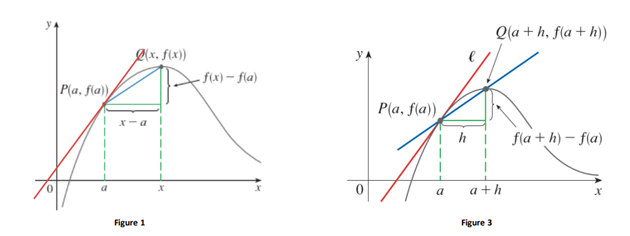
\includegraphics[width=12cm]{Def of Defferentiation.png}
    \end{center}

    \item Differentiable Failure\\
    \hspace*{2em} For a differentiable function, it must be \underline{continuous} and \underline{smooth}, the following conditions are those which don't meet these criteria.
    \begin{multicols}{2}
        \begin{enumerate}[(1)]
            \item Break Point
            \item Oscillation
            \item Sharp Point
            \item Sharp Turn
        \end{enumerate}
    \end{multicols}
    \item Differentiation of Trigonometric Functions\\
    Basic Trigonometric Functions:
    \begin{multicols}{2}
        \begin{enumerate}[i.]
            \item $sin'(x)=cos(x)$
            \item $cos'(x)=-sin(x)$
            \item $tan'(x)=sec^2(x)$
            \item $sec'(x)=sec(x)\cdot tan(x)$
            \item $csc'(x)=-csc(x)\cdot cot(x)$
            \item $cot'(x)=-csc^2(x)$
        \end{enumerate}
    \end{multicols}
\newpage
        \item Intermediate form for special trigonometric functions
        \begin{enumerate}[i.]
            \item $\lim\limits_{\theta\to0}\frac{sin(\theta)}{\theta}=1$\\
            Proofing method: Geometric argument\\
            \rightline{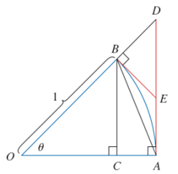
\includegraphics[width=4cm]{Geometric Argument.png}\hspace{3cm}}
            \\
            \\
            \item $\lim\limits_{\theta\to0}\frac{cos(\theta)-1}{\theta}=0$\\
            Proofing method: Trigonometric identity\\
            \\
            \\
            \\
            \\
            \\
            \item CH4.4 L'Hospital's Rule (For Refernce)\\
            L'Hospital's Rule can be applied only when limit encounters indeterminate form, which is often shown as $\frac{\infty}{\infty}$ or $\frac{0}{0}$ in fractional form.\\
            \\
            \textbf{\textit{Example 1}}\\
            Solve $\lim\limits_{x\to0}\frac{sin(x)}{\sqrt{x+1}-\sqrt{1-x}}$\\
            \\
            \\
            \\
            
            \textbf{\textit{Example 2}}\\
            Solve $\lim\limits_{x\to0}\frac{x+xcos(x)}{sin(x)\cdot cos(x)}$\\
            \\
            \\
            \\
            
\newpage
            \textbf{\textit{Exercise 1}}\\
            Solve $\lim\limits_{x\to\frac{\pi}{4}}\frac{sin(x)-sin(\pi/4)}{x-\pi/4}$\\
            \\
            \\
            \\
            \\
            \\
            \textbf{\textit{Exercise 2}}\\
            Solve $\lim\limits_{x\to0}cos(x)^{1/x^2}$\\
            \\
            \\
            \\
            \\
            \\
        \end{enumerate}
            \item Chain Rule\\
            \hspace*{2em}In previous chapters, we’ve already discussed derivatives of non-composite functions, however when dealing with derivatives of composite functions, the situation becomes more complicated, when solving these types of problems, chain rule is applied.\\
            \hspace*{2em}Suppose $F(x)$ is a composite function composed of $f(x)$, $g(x)$, and $h(x)$, then:
            $$F(x)=f(g(h(x)))$$
            \hspace*{2em}While differentiating composite functions, chain rule states that we differentiate the function from the outer ones to the inner ones respectively and multiply these results altogether. If we take $F(x)$ for example, its differentiation will be:
            $$F'(x)=f'(g(h(x)))\cdot g'(h(x))\cdot h'(x)$$\\
            \textbf{\textit{Example 1}}\\
            Differentiate $f(x)=(9x^2-6x+2)5^{x^3}$\\
            \\
            \\
            \\
            \textbf{\textit{Example 2}}\\
            Differentiate $f(x)=(\frac{3-2x}{1+sin(3x)})$\\
            \\
            \\
            \\
            \\
            \\
            \textbf{\textit{Example 3}}\\
            Differentiate $f(x)=sec^2(x\cdot tan(sec(x)\cdot tan(x)))$\\
            \\
            \\
            \\
            \\
            \\
            \textbf{\textit{Exercise 1}}\\
            Differentiate $f(x)=\sqrt{x\sqrt{x+\sqrt{x}}}$\\
            \\
            \\
            \\
            \\
            \\
            \textbf{\textit{Exercise 2}}\\
            Differentiate $f(x)=(e^{-6x}+sec(2-x))^3$\\
            \\
            \\
            \\
            \\
            \\
            \textbf{\textit{Exercise 3}}\\
            Differentiate $f(x)=ln(sin(x))-(x^4-3x)^{10}$
            \\
            \\
            \\
            \\
            \\
\end{enumerate}

\end{document}